\section{代数基本定理}
\label{section:ch09-sec56}

每一个实系数或复系数的 $n$ 次方程
\[
x^{n}+a_{n-1}x^{n-1}+\cdots+a_{1}x+a_{0}=0
\]
有 $n$ 个根 (几重根就称为几个根). 这是复数的一个基本性质. 可能读者在中学代数学课程中就见过这个定理, 但那时却无法证明它.

事实上, 这个证明是相当困难的. 最难的部分是证明次数为正数时, 方程至少有一个根. 对此有许多不同的证法. 可以用代数的技巧, 然而代数的证明既长又费力. 也可以用复变函数论的方法, 在复变函数论中, 这个定理是 Liouville 定理的明显推论. 而我们这里给出的证明相当简单, 它作为圆周基本群计算的简单推论.

\begin{theorem}[代数基本定理]
\label{theorem:ch09-sec56-56-1}
实系数或复系数的 $n>0$ 次方程
\[
x^{n}+a_{n-1}x^{n-1}+\cdots+a_{1}x+a_{0}=0
\]
至少有一个 (实的或复的) 根.
\end{theorem}

\par
\begin{figure}[htbp]
\centering
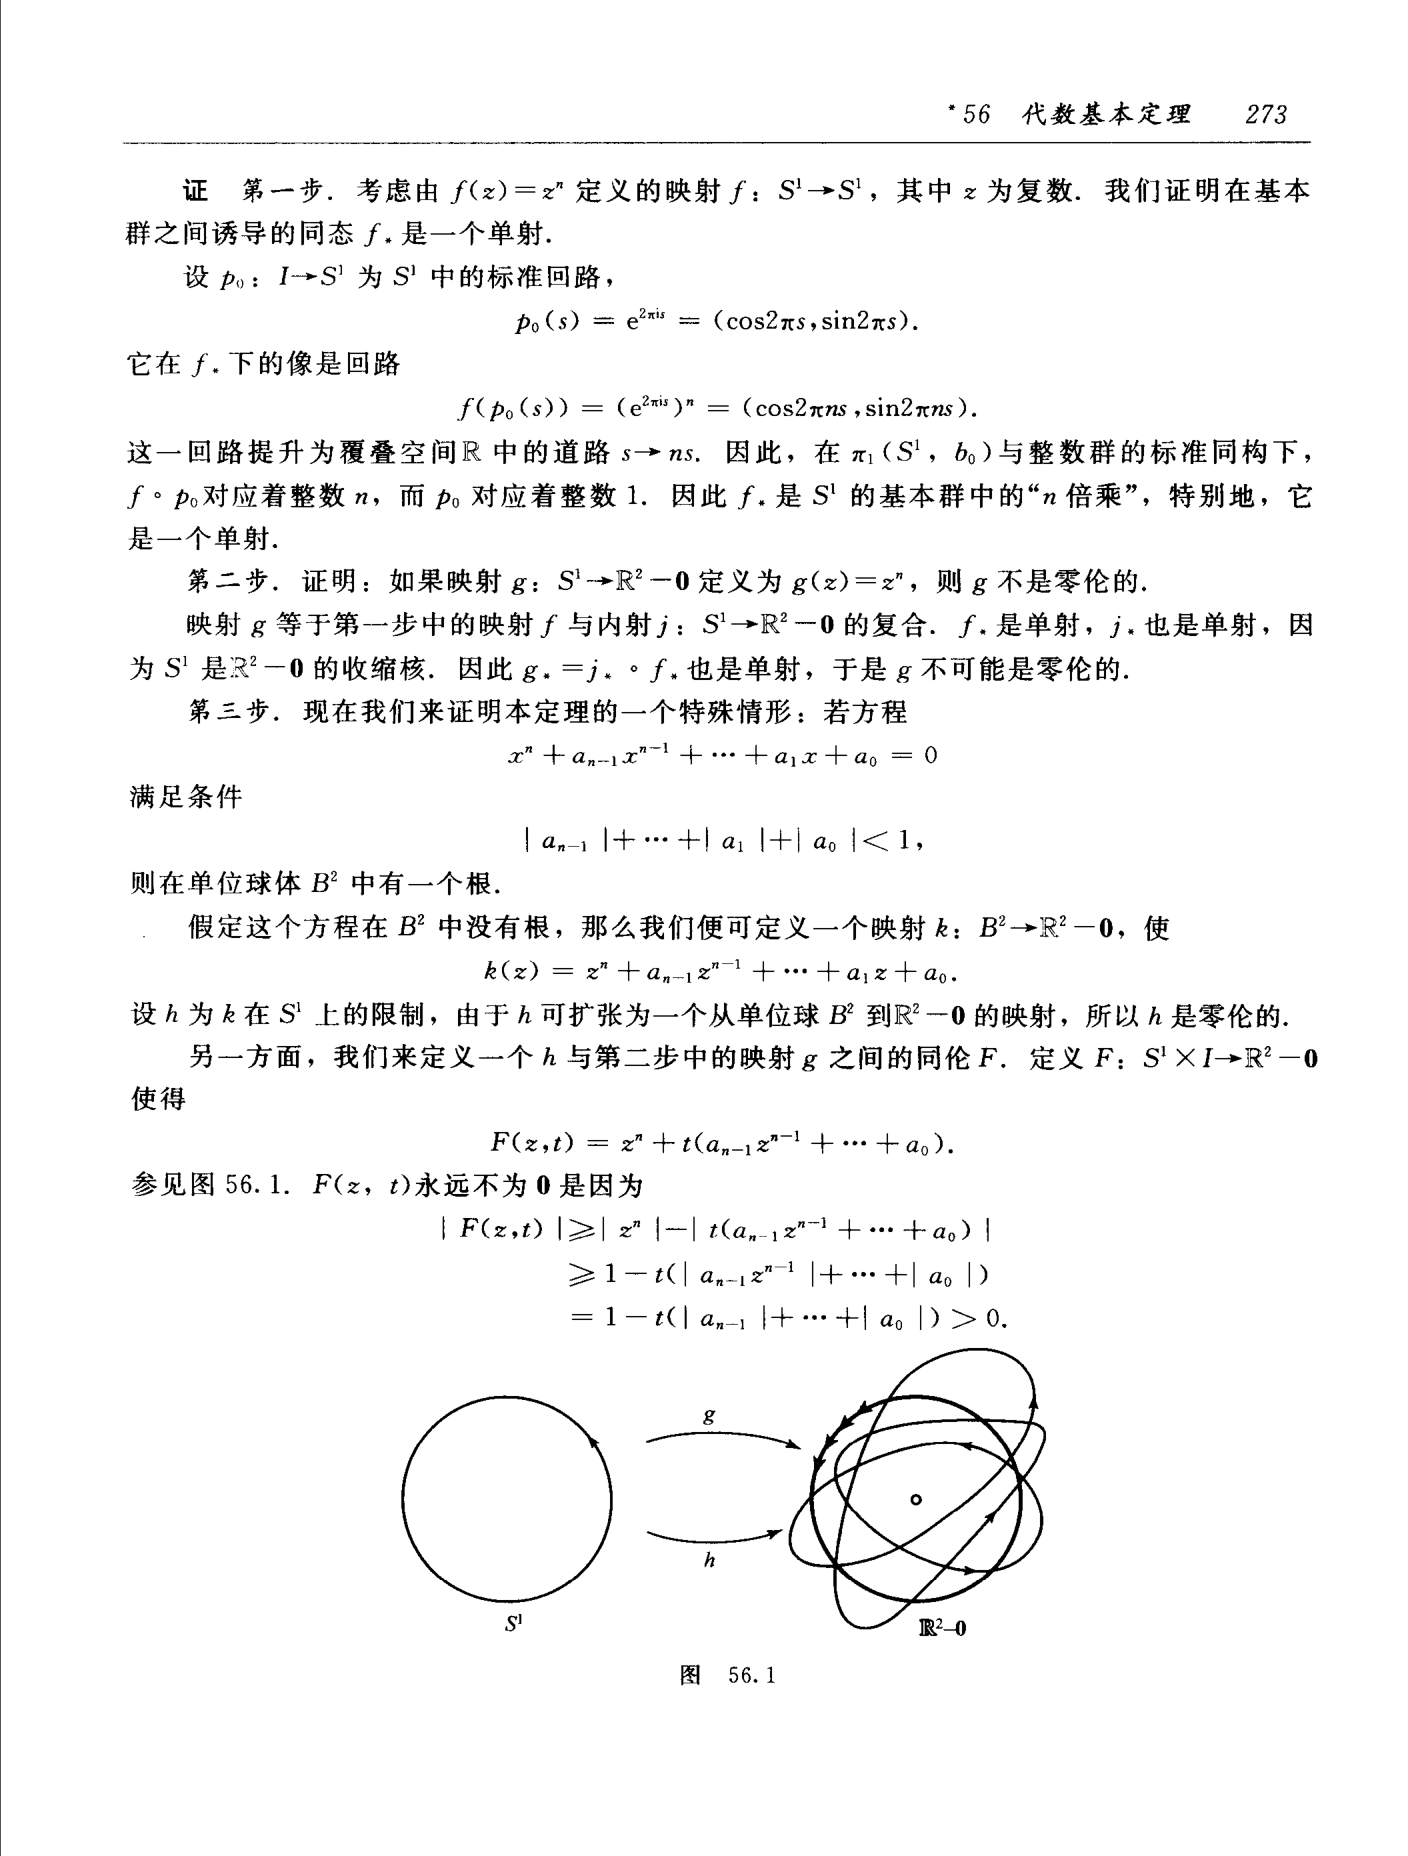
\includegraphics[width=0.6\textwidth]{image/fig-56-1.png}
\caption{代数基本定理的证明.}
\label{figure:ch09-fig-56-1}
\end{figure}

\begin{proof}
\textbf{第一步.} 考虑由 $f(z)=z^n$ 定义的映射 $f\colon S^{1}\to S^{1}$, 其中 $z$ 为复数. 我们证明在基本群之间诱导的同态 $f_*$ 是一个单射.

设 $p_0\colon I\to S^{1}$ 为 $S^{1}$ 中的标准回路,
\[
p_{0}(s)=\mathrm{e}^{2\pi\mathrm{i}s}=(\cos 2\pi s,\sin 2\pi s).
\]
它在 $f_*$ 下的像是回路
\[
f(p_{0}(s))=(\mathrm{e}^{2\pi\mathrm{i}s})^{n}=(\cos 2\pi ns,\sin 2\pi ns).
\]
这一回路提升为覆叠空间 $\mathbb{R}$ 中的道路 $s\mapsto ns$. 因此, 在 $\pi_1(S^{1},b_0)$ 与整数群的标准同构下, $f\circ p_0$ 对应着整数 $n$, 而 $p_0$ 对应着整数 $1$. 因此 $f_*$ 是 $S^{1}$ 的基本群中的"$n$ 倍乘", 特别地, 它是一个单射.

\textbf{第二步.} 证明: 如果映射 $g\colon S^{1}\to\mathbb{R}^{2}-\boldsymbol{0}$ 定义为 $g(z)=z^n$, 则 $g$ 不是零伦的.

映射 $g$ 等于第一步中的映射 $f$ 与内射 $j\colon S^{1}\to\mathbb{R}^{2}-\boldsymbol{0}$ 的复合. $f_*$ 是单射, $j_*$ 也是单射, 因为 $S^{1}$ 是 $\mathbb{R}^{2}-\boldsymbol{0}$ 的收缩核. 因此 $g_*=j_*\circ f_*$ 也是单射, 于是 $g$ 不可能是零伦的.

\textbf{第三步.} 现在我们来证明本定理的一个特殊情形: 若方程
\[
x^{n}+a_{n-1}x^{n-1}+\cdots+a_{1}x+a_{0}=0
\]
满足条件
\[
|a_{n-1}|+\cdots+|a_{1}|+|a_{0}|<1,
\]
则在单位球体 $B^{2}$ 中有一个根.

假定这个方程在 $B^{2}$ 中没有根, 那么我们便可定义一个映射 $k\colon B^{2}\to\mathbb{R}^{2}-\boldsymbol{0}$, 使
\[
k(z)=z^{n}+a_{n-1}z^{n-1}+\cdots+a_{1}z+a_{0}.
\]
设 $h$ 为 $k$ 在 $S^{1}$ 上的限制, 由于 $h$ 可扩张为一个从单位球 $B^{2}$ 到 $\mathbb{R}^{2}-\boldsymbol{0}$ 的映射, 所以 $h$ 是零伦的.

另一方面, 我们来定义一个 $h$ 与第二步中的映射 $g$ 之间的同伦 $F$. 定义 $F\colon S^{1}\times I\to\mathbb{R}^{2}-\boldsymbol{0}$ 使得
\[
F(z,t)=z^{n}+t(a_{n-1}z^{n-1}+\cdots+a_{0}).
\]
参见图 \cref{figure:ch09-fig-56-1}. $F(z,t)$ 永远不为 $\boldsymbol{0}$ 是因为
\[
\begin{aligned}
|F(z,t)|&\geqslant |z^{n}|-|t(a_{n-1}z^{n-1}+\cdots+a_{0})|\\
&\geqslant 1-t(|a_{n-1}z^{n-1}|+\cdots+|a_{0}|)\\
&=1-t(|a_{n-1}|+\cdots+|a_{0}|)>0.
\end{aligned}
\]


\textbf{第四步.} 现在来证明一般情形. 对于给定的多项式方程
\[
x^{n}+a_{n-1}x^{n-1}+\cdots+a_{1}x+a_{0}=0,
\]
选取一个实数 $c>0$, 然后取变换 $x=cy$, 则得到方程
\[
(cy)^{n}+a_{n-1}(cy)^{n-1}+\cdots+a_{1}(cy)+a_{0}=0,
\]
也就是
\[
y^{n}+\frac{a_{n-1}}{c}y^{n-1}+\cdots+\frac{a_{1}}{c^{n-1}}y+\frac{a_{0}}{c^{n}}=0.
\]
如果最后这个方程有一个根 $y=y_0$, 那么最初的方程就有根 $x_0=cy_0$. 所以, 只要将 $c$ 取得足够大, 使得
\[
\left|\frac{a_{n-1}}{c}\right|+\left|\frac{a_{n-2}}{c^{2}}\right|+\cdots+\left|\frac{a_{1}}{c^{n-1}}\right|+\left|\frac{a_{0}}{c^{n}}\right|<1,
\]
那么, 由第三步中研究过的特殊情形, 本定理证明完成.
\end{proof}

\subsection*{习题}

\begin{exercise}
给定一个实系数或复系数的方程
\[
x^{n}+a_{n-1}x^{n-1}+\cdots+a_{1}x+a_{0}=0.
\]
证明: 当 $|a_{n-1}|+\cdots+|a_{1}|+|a_{0}|<1$ 时, 这个方程的所有根都在单位球 $B^{2}$ 的内部. [提示: 设 $g(x)=1+a_{n-1}x+\cdots+a_{1}x^{n-1}+a_{0}x^n$, 并证明当 $x\in B^{2}$ 时, $g(x)\neq 0$.]
\end{exercise}

\begin{exercise}
找出一个以原点为圆心的圆周, 使得它包含方程 $x^7+x^2+1=0$ 的全部根.
\end{exercise}